\chapter{Detalles de implementación y experimentos}\label{chapter:implementation}

Este capítulo presenta los métodos, técnicas, detalles e hiperparámetros utilizados en la implementación general del modelo y específica de cada experimento.

\section*{Configuraciones generales}

El código desarrollado en la implementación de este modelo en púbico y se puede descargar en github en el repositorio \href{https://github.com/deborahfam/Thesis}{github.com/deborahfam/Thesis} en la carpeta llamada \textit{pipelines}. Cada pipeline es un archivo \textit{.ipynb}. Adelante se describen herramientas y tecnologías que fueron utilizadas en el proyecto:

\section*{Herramientas y Tecnologías}

\begin{itemize}
   \item \textbf{Frameworks de Desarrollo:}
   \begin{itemize}
       \item TensorFlow: Framework principal para la construcción y entrenamiento de modelos de machine learning y redes neuronales profundas.
   \end{itemize}

   \item \textbf{APIs y bibliotecas de TensorFlow:}
   \begin{itemize}
       \item Keras: API de alto nivel para la construcción y entrenamiento de modelos en TensorFlow.
       \item tf.keras.layers: Conjunto de capas predefinidas para la construcción de modelos.
       \item tf.keras.optimizers: Algoritmos de optimización como Adam y Adamax.
       \item tf.keras.metrics: Métricas de evaluación como categorical\_crossentropy.
       \item tf.keras.regularizers: Técnicas de regularización como L1 y L2.
       \item tf.keras.preprocessing.image: Herramientas de preprocesamiento y aumento de imágenes.
       \item tf.keras.models: Herramientas para la creación y carga de modelos.
   \end{itemize}

   \item \textbf{Manipulación de Datos:}
   \begin{itemize}
       \item NumPy: Manejo de \textit{arrays} y matrices de números n-dimensionales.
       \item Pandas: Análisis y manipulación de datos estructurados.
   \end{itemize}

   \item \textbf{Utilidades de Sistema y Archivos:}
   \begin{itemize}
       \item Shutil: Operaciones de manejo de archivos.
       \item OS: Interacción con el sistema operativo.
   \end{itemize}

   \item \textbf{Visión por Computadora:}
   \begin{itemize}
       \item OpenCV (cv2): Procesamiento de imágenes y visión por computadora.
   \end{itemize}

   \item \textbf{Herramientas de Visualización de Datos:}
   \begin{itemize}
       \item Matplotlib: Creación de gráficos y visualizaciones.
       \item Seaborn: Visualización de datos estadísticos.
   \end{itemize}

   \item \textbf{Evaluación de Modelos:}
   \begin{itemize}
       \item Scikit-learn (sklearn): Herramientas para selección de modelos y evaluación.
   \end{itemize}

   \item \textbf{Procesamiento de Imágenes:}
   \begin{itemize}
       \item Pillow (PIL): Procesamiento de imágenes para aplicaciones Python.
   \end{itemize}

   \item \textbf{Herramientas de Progreso y Medición de Tiempo:}
   \begin{itemize}
       \item TQDM: Barras de progreso para loops.
       \item Time: Medición del tiempo de ejecución de código.
   \end{itemize}

   \item \textbf{Mejora de Interfaz y Presentación:}
   \begin{itemize}
       \item IPython: Mejoras interactivas y de visualización para Python, especialmente en cuadernos Jupyter.
   \end{itemize}
\end{itemize}


\subsection*{Carga, visualización y transformación de datos}

Lo primero realizado fue la importación y transformación los datos para el modelo. En el proceso de importación, para la carga de imágenes utilizamos \texttt{plt.imread} de la librería Matplotlib y \texttt{pd.read\_csv} de la librería Pandas para cargar los metadatos. Para la división del conjunto de datos en entrenamiento, validación y prueba se utilizó la función \texttt{train\_test\_split} de la librería Scikit-Learn con las variables \texttt{random\_state=123} y \texttt{shuffle=True}. Estas variables aseguran aleatoriedad en la división mezclando los datos antes de dividirlos y que la división sea reproducible. La división, como se expresó en capítulos anteriores es distinta en cada experimento y se especifican los parámetros utilizados luego en el capítulo.

Para la carga y procesamiento de imágenes se utilizó la clase \texttt{ImageDataGenerator} de Keras \brackcite{img_gen}. Esta clase facilita la creación de lotes de imágenes que se utilizan durante el entrenamiento y la evaluación de modelos de Machine Learning, especialmente en el contexto de redes neuronales. 

Las transformaciones aplicadas fueron las siguientes

\begin{table}[ht]
   \centering
   \begin{tabular}{lccc}
   \hline
   Parámetro & Descripción  & Valor \\ \hline
   rotation range & 	Rango de rotación & 20 grados \\
   width shift range & Rango de desplazamiento horizontal & 20\% \\
   height shift range & Rango de desplazamiento vertical & 20\% \\
   shear range & 	Rango de corte & 20\% \\
   zoom range & Rango de zoom & 20\% \\
   horizontal flip & Activación de volteo horizontal & verdadero \\
   fill mode & Modo de relleno para manejar los píxeles faltantes & nearest \\ \hline
   \end{tabular}
   \caption{Parámetros de aumento de datos.}
   \label{tab:data_augmentation_params}
   \end{table}
     

\section*{Preparación del modelo}

El siguiente fragmento de código siguiente detalla la creación y compilación de un modelo de aprendizaje profundo utilizando Keras, una API de alto nivel para construir y entrenar modelos en TensorFlow. El modelo se basa en EfficientNetB1. Para la compilación del mismo se hace uso de \texttt{model.compile}, con un callback personalizado para ajustar la tasa de aprendizaje y para entrenar utilizamos el \texttt{model.fit}.

\begin{lstlisting}[language=Python]
   model_name='EfficientNetB1'
   base_model=tf.keras.applications.EfficientNetB1(include_top=False, weights="imagenet",input_shape=img_shape, pooling='max')

   x=base_model.output
   x=keras.layers.BatchNormalization(axis=-1, momentum=0.99, epsilon=0.001 )(x)
   x = Dense(256, kernel_regularizer = regularizers.l2(l = 0.016),activity_regularizer=regularizers.l1(0.006),
                  bias_regularizer=regularizers.l1(0.006) ,activation='relu')(x)
   x=Dropout(rate=.45, seed=123)(x)

   output=Dense(class_count, activation='softmax')(x)
   model=Model(inputs=base_model.input, outputs=output)
   model.compile(Adamax(learning_rate=.001), loss='categorical_crossentropy', metrics=['accuracy'])
\end{lstlisting}

\subsection*{Detalles de Hiperparámetros y Configuración}

\begin{itemize}
   \item \textbf{Arquitectura del Modelo:} Se utiliza EfficientNetB1 preentrenado con pesos de ImageNet como base.
   \item \textbf{Tasa de Aprendizaje Inicial:} Establecida en $0.001$.
   \item \textbf{Regularización:} Aplicación de regularización L2 con $\lambda = 0.016$ y regularización L1 con $\lambda = 0.006$ para los pesos y sesgos.
   \item \textbf{Dropout:} Se implementa una tasa de dropout del 45\% para mitigar el sobre-ajuste.
   \item \textbf{Dimensiones de la Imagen:} $224 \times 224 \times 3$.
   \item \textbf{Optimizador:} Adamax.
   \item \textbf{Métrica de Evaluación:} La precisión (\textit{accuracy}) se utiliza como la métrica de evaluación principal.
   \item \textbf{Callbacks:} Se incorpora un ajuste de tasa de aprendizaje (LRA) con los siguientes parámetros
   \item \begin{itemize}
      \item \textbf{Epochs:} $40$.
      \item \textbf{Patience:} 1.      
      \item \textbf{Stop Patience:} 3.
      \item \textbf{Threshold:}  0.9.
      \item \textbf{Factor:} 0.5.      
      \item \textbf{Dwell:} True
      \item \textbf{Freeze:} False  
      \item \textbf{Batches:} $train\_steps = (len(train_gen.labels)/batch_size)$
   \end{itemize}
\end{itemize}

\begin{table}[ht]
   \centering
   \small
   \begin{tabular}{|c|p{10cm}|}
   \hline
   \textbf{Término} & \textbf{Descripción} \\
   \hline
   Epoch & Es una iteración completa sobre todo el conjunto de datos de entrenamiento. \\
   \hline
   Loss (Pérdida) & Es una medida de cuán bien el modelo está realizando sus predicciones. Los valores decrecientes indican una mejora en el aprendizaje. \\
   \hline
   Accuracy (Precisión) & Muestra el porcentaje de etiquetas que el modelo predice correctamente para el conjunto de entrenamiento. \\
   \hline
   V loss (Pérdida de Validación) & Es similar a la pérdida, pero se calcula sobre un conjunto de datos que no se utiliza para el entrenamiento. \\
   \hline
   V acc (Precisión de Validación) & Muestra el porcentaje de etiquetas que el modelo predice correctamente para el conjunto de datos de validación. \\
   \hline
   LR (Learning Rate) & La tasa de aprendizaje dicta cuánto se ajustan los pesos del modelo en cada actualización. \\
   \hline
   Next LR (Próxima Learning Rate) & Indica la próxima tasa de aprendizaje planificada. La adaptación de la tasa de aprendizaje puede ayudar a evitar el estancamiento y mejorar la convergencia. \\
   \hline
   Monitor & Muestra la métrica que se está utilizando para monitorizar el rendimiento del modelo. Cambia de \textit{accuracy} a \textit{val loss}, lo que probablemente indica que el cambio se hizo para evitar el sobre'ajuste. \\
   \hline
   Duration (Duración) & Tiempo que tardó cada epoch en completarse. Importante para evaluar la eficiencia del entrenamiento. \\
   \hline
   \end{tabular}
   \caption{Descripción de términos clave en el entrenamiento de modelos de aprendizaje automático.}
   \label{table:terminology}
   \end{table}

\section{Capas adicionales y regularización}
   
   Para ajustar y optimizar el modelo de EfficientNetB1, se añaden capas adicionales:
   
   \subsection{Normalización por lotes}
   
   Esta capa se define con un \textit{eje de normalización} establecido en $-1$, lo que indica que la normalización se aplica a lo largo del último eje en el tensor de entrada. Además, se configura un \textit{momentum} de $0.99$ y un valor de \textit{epsilon} de $0.001$. El alto valor de \textit{momentum} ayuda a mantener la estabilidad de las medias y varianzas móviles a lo largo del entrenamiento, mientras que el pequeño valor de epsilon evita divisiones por cero, asegurando así cálculos numéricos estables \brackcite{regularization}.
   
   \subsection{Capa densa}
   
   Se integra una capa densa con $256$ neuronas, que juega un papel clave en la síntesis de las características aprendidas por el modelo. Se utiliza un regularizador L2 con un \textit{lambda} de $0.016$ para los pesos de la capa, lo que ayuda a penalizar y controlar el tamaño de los pesos, reduciendo así el riesgo de sobre-ajuste. Además, tanto el regularizador de actividad como el regularizador de bias se configuran con un regularizador L1 con un \textit{lambda} de $0.006$. Este enfoque impone una penalización en los pesos y los sesgos, promoviendo un modelo más simple y disperso. La función de activación utilizada es \textit{ReLU} , conocida por su eficacia en la introducción de no linealidad en el modelo, lo que permite aprender relaciones complejas entre las características \brackcite{dense}.
   
   \subsection{Dropout}
   
   En la arquitectura del modelo, se integra una capa de \textit{dropout} para aumentar la robustez y prevenir el sobre-ajuste. Esta capa se configura con una tasa de desactivación del 45\% , lo que significa que, durante el entrenamiento, el 45\% de las neuronas se desactivarán aleatoriamente en cada paso. 
   
   En una primera iteración del algoritmo tuvo una tasa de desactivación más baja. Luego de varias iteraciones se concluyó que se necesitaba un algoritmo de clasificación que estudiara más a detalle la data fomentando así una mejor generalización y reduciendo el riesgo de sobre-ajuste en el proceso de aprendizaje. Dado esto, en esto se aumenta la tasa y se obtienen mejores resultados.
   
   Para asegurar la reproducibilidad, se establece una semilla(seed) $123$. Esta introducción de aleatoriedad ayuda a que el modelo no dependa excesivamente de ninguna característica o neurona específica \brackcite{dropout}.
   
   \subsection{Capa de salida}
   
   La capa de salida utiliza una activación \textit{softmax} para transformar las salidas del modelo en probabilidades de pertenencia a cada clase. Esto clasifica las entradas en categorías distintas, proporcionando probabilidades para cada clase, lo cual es esencial en la clasificación multi-clase.
   
   \subsection{Optimización}
   
   Para el proceso de entrenamiento se utiliza el optimizador \textit{Adamax} \brackcite{adamax}. Este es una variante del conocido optimizador Adam, que combina las ventajas de los métodos adaptativos de tasa de aprendizaje con una implementación más robusta en entornos con gradientes dispersos, lo cual es común en imágenes médicas 
   
   La función de pérdida elegida es la \textit{categorical crossentropy} \brackcite{vitalflux_categorical_crossentropy}, idónea para problemas de clasificación multi-clase. Se configura el modelo para minimizarla y se rastrea la precisión como métrica principal.

\section{Experimentos}

Como se había expresado previamente, se llevaron a cabo una serie de experimentos de los cuales analizaremos los siguientes para la distribución y normalización de datos. La metodología general para ambos experimentos coincide, en ambos se utiliza una red convolucional, EfficientNetB1 y capas adicionales.

\subsection{Experimento 1: Evaluación de la eficiencia de la división asimétrica de datos en la clasificación de imágenes de cáncer de piel}

Este experimento se realiza con la intesión de utilizar una técnica clásica de división de datos para el entrenamiento y test del algoritmo implementado para la resolución del problema, teniendo en cuenta que la distribución de datos es importante en cuestión de efectividad de los algoritmos. Se centra en una división de datos altamente asimétrica, con un enfoque predominante en el conjunto de entrenamiento. La técnica de \textit{dummy split} se emplea para mantener proporciones consistentes entre los conjuntos de validación y prueba. A esta división se le aplica luego un determinado peso para que el algoritmo preste especial atención a las clases menos representadas. 

\subsection*{Distribución de datos}

En este experimento de las herramientas que se utiliza para hacer la división se hace uso del \textit{dummy split}  para mantener la proporción deseada entre validación y prueba. Se escoge la siguiente distribución de datos para realizar una prueba de datos en la que existiera desproporción y se entrenara el modelo para ver fallas e índices de sobre-ajuste y en otras versiones mejorar la distribución de datos del modelo. La distribución fue la siguiente:

\begin{table}[ht]
   \centering
   \begin{tabular}{lcc}
   \hline
   \textbf{Diagnostic category} & \textbf{Porcentaje} & \textbf{Cantidad de datos} \\
   \hline
   Entrenamiento       & 95\% & $9514$ \\
   Validación      & 2.5\% & $251$  \\
   Prueba      & 2.5\% & $251$  \\ \hline
   \end{tabular}
   \caption{Distribución de los conjuntos de entrenamiento, validación y prueba.}
   \label{table:data_distribution_e1}
   \end{table}

   Por lo que la division de datos por clase quedaría de la siguiente forma:

   \begin{table}[ht]
      \centering
      \begin{tabular}{lccc}
      \hline
      \textbf{Diagnostic category} & \textbf{Entrenamiento} & \textbf{Validación} & \textbf{Prueba} \\
      \hline
      NV       & 300 & 158 & 163 \\
      MEL      & 300 & 25  & 35  \\
      BKL      & 300 & 34  & 30  \\
      DF       & 115 & 5   & 3   \\
      AKIEC    & 300 & 11  & 7   \\
      BCC      & 300 & 16  & 10  \\
      VASC     & 142 & 1   & 3   \\ \hline
      \end{tabular}
      \caption{Experimento 1: Distribución de imágenes de cáncer de piel en los conjuntos de entrenamiento, test y validación.}
      \label{table:train_test_validate_e1}
      \end{table}
   
\subsubsection*{Generadores de datos y preprocesamiento}

Se establece para este un tamaño objetivo de muestras por clase ($300$ en este caso), y se utiliza un bucle para iterar a través de cada clase única.

\begin{table}[ht]
   \centering
   \begin{tabular}{lccc}
   \hline
   Diagnostic category & Sampling  \\ \hline
   AKIEC & 300 \\
   BCC & 300 \\
   BKL & 300 \\
   DF & 115 \\
   MEL & 300 \\
   NV & 300 \\
   VASC & 142 \\ \hline
   \end{tabular}
   \caption{Distribución de muestras por categoría después del sobre-muestreo.}
   \label{tab:sampling_distribution_1}
   \end{table}


Como se evidencia anteriormente, al separar la data en clases el conjunto se mantiene desbalanceado. Se hace necesario aplicar un método llamado \textit{Class Weighting} para compensar este desbalanceo. Este método consiste en asignar un peso a cada clase inversamente proporcional a su frecuencia. De esta manera, las clases con menor representación tendrán un mayor peso y las clases con mayor representación tendrán un menor peso. Esto permite que el modelo se entrene de manera más equilibrada y que no se sesgue hacia las clases con mayor representación.

\begin{table}[ht]
   \centering
   \begin{tabular}{lccc}
   \hline
   Diagnostic category & Sampling  & Weighting\\ \hline
   AKIEC & 300 & 1.00\\
   BCC & 300 & 1.00\\
   BKL & 300 & 1.00\\
   DF & 115 & 2.60\\
   MEL & 300 & 1.00\\
   NV & 300 & 1.00\\
   VASC & 142 & 2.11\\ \hline
   \end{tabular}
   \caption{Distribución de muestras con peso asignado.}
   \label{tab:weighting_distribution}
   \end{table}


\subsection{Experimento 2: Análisis de la estratificación de datos en la clasificación de imágenes de cáncer de piel}

Este experimento explora la estratificación de datos para mantener una distribución uniforme de etiquetas en cada conjunto de datos. Dado que la distribución anterior muestra un sobre-ajuste, se opta por una proporción de los conjuntos de datos es más equilibrada en comparación con el Experimento 1, lo que ofrece \textit{insights} sobre la importancia de la distribución equitativa de datos en el entrenamiento y evaluación de modelos.

\subsection*{Distribución de datos}

Se utiliza \textit{stratify} en ambas divisiones para mantener la distribución de etiquetas \textit{label} en cada conjunto. Se calcula la proporción del conjunto de prueba sobre la suma del conjunto de test y el de validación. La distribución de datos fue la siguiente:

   \begin{table}[ht]
      \centering
      \begin{tabular}{lcc}
      \hline
      \textbf{Diagnostic category} & \textbf{Porcentaje} & \textbf{Cantidad de datos} \\
      \hline
      Entrenamiento       & 70\% &  $7010$ \\
      Validación      & 15\% & $1502$  \\
      Prueba      & 15\% & $1503$  \\ \hline
      \end{tabular}
      \caption{Distribución de los conjuntos de entrenamiento, validación y prueba.}
      \label{table:data_distribution_e2}
      \end{table}

Luego este quedaría distribuido en datos de entrenamiento, test y  validación por clase de la siguiente forma:
   \begin{table}[ht]
      \centering
      \begin{tabular}{lccc}
      \hline
      \textbf{Diagnostic category} & \textbf{Training} & \textbf{Validation} & \textbf{Testing} \\
      \hline
      NV    & 500 & 1006 & 1006 \\
      MEL   & 500 & 167  & 167  \\
      BKL   & 500 & 165  & 165  \\
      DF    & 500 & 17   & 17   \\
      AKIEC & 500 & 49   & 49   \\
      BCC   & 500 & 77   & 77   \\
      VASC  & 500 & 21   & 22   \\
      \hline
      \end{tabular}
      \caption{Experimento 2: Distribución de imágenes de cáncer de piel en los conjuntos de entrenamiento, test y validación.}
      \label{tab:train_test_validate_e2}
      \end{table}
 
\subsubsection*{Generadores de datos y preprocesamiento}

Se establece también un tamaño objetivo de muestras por clase ($500$). Se itera sobre cada clase, y se realiza un re-muestreo con reemplazo para grupos menores al tamaño deseado y sin reemplazo para los grupos que ya alcanzan o superan el tamaño deseado. 
En este experimento, a diferencia del anterior, en cada clase se alcanza la misma cantidad de muestras, por lo que no es necesario aplicar \textit{Class Weighting}.

\section{Resultados de los experimentos}

En esta sección se presenta un marco experimental y se realiza un análisis comparativo para evaluar la efectividad de los experimentos realizados. Para ello se emplean gráficos para visualizar la pérdida y la precisión tanto de entrenamiento como de validación a lo largo de las épocas (iteraciones), marcando la época con menor pérdida de validación y mayor precisión de validación.

Se genera también un gráfico de barras que muestra la distribución de errores por clase en el conjunto de pruebas. Además, se genera una matriz de confusión y un informe de clasificación que incluye precisión, recuperación (recall), puntuación F1 y soporte para cada clase. Al final del entrenamiento, se evalúa el modelo en el conjunto de pruebas y se obtiene la precisión del mismo. El modelo con mayor eficiencia luego de varios ajustes tuvo una eficacia cercana al 87\%.

La tabla 4.1 al final del capítulo describe las métricas utilizadas para la evaluación del modelo.

\subsection*{Pérdida y precisión (loss y accuracy)}

En el primer experimento se observa que la precisión de entrenamiento aumenta con cada epoch, la pérdida de entrenamiento disminuye consistentemente y la tasa de aprendizaje permanece constante al principio y luego disminuye para afinar el entrenamiento a medida que el modelo comienza a converger, lo cual indica que el modelo esta entrenando de forma correcta. Sin embargo, la división asimétrica de datos en este experimento influye en el aprendizaje del modelo. El uso de división asimétrica puede estar causando que el modelo esté sesgado hacia clases con más muestras, afectando la precisión general y la capacidad de generalizar. Esto se evidencia dado que, a pesar de la disminución de la pérdida de validación y el aumento de la precisión de validación, la notable diferencia entre la precisión de entrenamiento y la precisión de validación podría indicar un potencial sobre-ajuste.

    \begin{table}[ht]
      \small
      \begin{center}
          \begin{tabular}{|c|c|c|c|c|c|c|c|} \hline
          E & Loss & Acc & V loss & V acc & LR & M & Batch \\ \hline
          1 & 9.587 & 40.581 & 8.95658 & 56.800 & $10^{-2}$ & acc & 85.25 \\ \hline
          2 & 7.798 & 67.615 & 7.67235 & 66.800 & $10^{-2}$ & acc & 21.72 \\ \hline
          3 & 6.884 & 79.340 & 6.96014 & 69.600 & $10^{-2}$ & acc & 22.56 \\ \hline
          4 & 6.214 & 87.365 & 6.35865 & 71.200 & $10^{-2}$ & acc & 25.81 \\ \hline
          5 & 5.646 & 91.690 & 5.94812 & 75.200 & $10^{-2}$ & vloss & 23.08 \\ \hline
          6 & 5.172 & 92.999 & 5.44954 & 76.800 & $10^{-2}$ & vloss & 23.23 \\ \hline
        %   7 & 4.735 & 94.479 & 5.06016 & 76.400 & $10^{-2}$ & vloss & 23.19 \\ \hline
        %   8 & 4.334 & 96.528 & 4.73837 & 76.800 & $10^{-2}$ & vloss & 22.90 \\ \hline
        %   9 & 3.969 & 97.211 & 4.33689 & 77.200 & $10^{-2}$ & val\_loss & 22.74 \\ \hline
        %   10 & 3.631 & 98.008 & 4.15826 & 74.000 & $10^{-2}$ & val\_loss & 22.56 \\ \hline
        %   11 & 3.315 & 98.406 & 3.89153 & 73.600 & $10^{-2}$ & val\_loss & 23.11 \\ \hline
          \dots & \dots & \dots & \dots & \dots & \dots & \dots & \dots \\ \hline
          34 & 0.627 & 99.886 & 1.24470 & 76.800 & 0.00013 & val\_loss & 23.30 \\ \hline
          \end{tabular}
          \caption{Estadísticas básicas del modelo del experimento 1.}
      \end{center}\label{fig:estadisticas_p1}
  \end{table}

  En el experimento 2 se utiliza la estratificación de datos para garantizar que cada clase este representada de manera proporcional. Similar al Experimento 1, en el Experimento 2 también se observa una disminución constante en la pérdida de entrenamiento (Loss) con cada epoch. La pérdida de entrenamiento (Loss) muestra una disminución significativa desde la primera hasta la última epoch registrada, pasando de 8.418 a 0.406. Esto indica un aprendizaje efectivo y una mejora continua en la capacidad del modelo para predecir con precisión las clases. La precisión (Acc), que comienza en 48.371\% y alcanza el 98.057\%, corrobora esta mejora constante. A diferencia del Experimento 1, la pérdida de validación (V loss) en este experimento, aunque también muestra una tendencia descendente, tiene una alineación más estrecha entre la precisión de entrenamiento y la precisión de validación. La pérdida de validación disminuye de manera más consistente y la precisión de validación es comparativamente más alta que en el Experimento 1, lo que indica una mejor capacidad de generalización.
    
\begin{table}[ht]
    \small
    \begin{center}
        \begin{tabular}{|c|c|c|c|c|c|c|c|} \hline
        E & Loss & Acc & V loss & V acc & LR & M & Batch \\ \hline
        1 & 8.418 & 48.371 & 7.41700 & 66.911 & $10^{-2}$ & accuracy & 184.55 \\ \hline
        2 & 6.362 & 69.943 & 5.81767 & 69.907 & $10^{-2}$ & accuracy & 107.94 \\ \hline
        3 & 5.110 & 77.686 & 4.76153 & 72.969 & $10^{-2}$ & accuracy & 106.30 \\ \hline
        4 & 4.181 & 81.371 & 3.86405 & 78.362 & $10^{-2}$ & accuracy & 104.60 \\ \hline
        5 & 3.417 & 84.771 & 3.25588 & 77.097 & $10^{-2}$ & accuracy & 101.90 \\ \hline
        6 & 2.777 & 87.314 & 2.70253 & 78.495 & $10^{-2}$ & accuracy & 101.85 \\ \hline
        % 7 & 2.247 & 90.143 & 2.24392 & 80.360 & $10^{-2}$ & val\_loss & 101.98 \\ \hline
        % 8 & 1.819 & 91.143 & 1.98878 & 77.364 & $10^{-2}$ & val\_loss & 101.74 \\ \hline
        % 9 & 1.464 & 92.543 & 1.70207 & 77.896 & $10^{-2}$ & val\_loss & 101.27 \\ \hline
        % 10 & 1.197 & 94.000 & 1.43860 & 81.225 & $10^{-2}$ & val\_loss & 101.71 \\ \hline
        % 11 & 0.992 & 94.000 & 1.24007 & 81.358 & $10^{-2}$ & val\_loss & 101.23 \\ \hline
        \dots & \dots & \dots & \dots & \dots & \dots & \dots & \dots \\ \hline
        22 & 0.406 & 98.057 & 0.81854 & 83.955 & 0.00006 & val\_loss & 101.18 \\ \hline
        \end{tabular}
        \caption{Estadísticas básicas del modelo del experimento 2.}
    \end{center}\label{fig:estadisticas_p2}
\end{table}
 
Las tablas 4.1 y 4.2 corresponde a la evaluación del experimento 1 y 2 respectivamente. Las tablas completas se pueden observar al final del capítulo, tablas 3.12 y 3.13.

\subsection*{Curva de aprendizaje}

Los análisis expuestos también se ven evidenciados en los gráficos de curvas de aprendizaje generados. Cada figura a continuación muestra dos gráficos, uno de pérdida y otro de precisión respectivamente, a lo largo de los epoch de entrenamiento y validación de cada experimento.

En el primer experimento la pérdida de entrenamiento (línea roja) y la pérdida de validación (línea verde) disminuyen con el tiempo, lo que indica que el modelo está aprendiendo. La mejor epoch basada en la pérdida de validación es la 31, marcada por un punto azul. La precisión de entrenamiento (línea roja) es casi perfecta, cercana al 100\%, lo que puede ser un indicador de sobre-ajuste. La precisión de validación (línea verde) mejora pero tiene una variabilidad considerable y alcanza su punto más alto en la epoch 29, también marcada con un punto azul. Hay una brecha notable entre la precisión de entrenamiento y validación, lo que puede ser un signo de que el modelo no está generalizando bien.

\begin{figure}[ht]%
    \begin{center}
        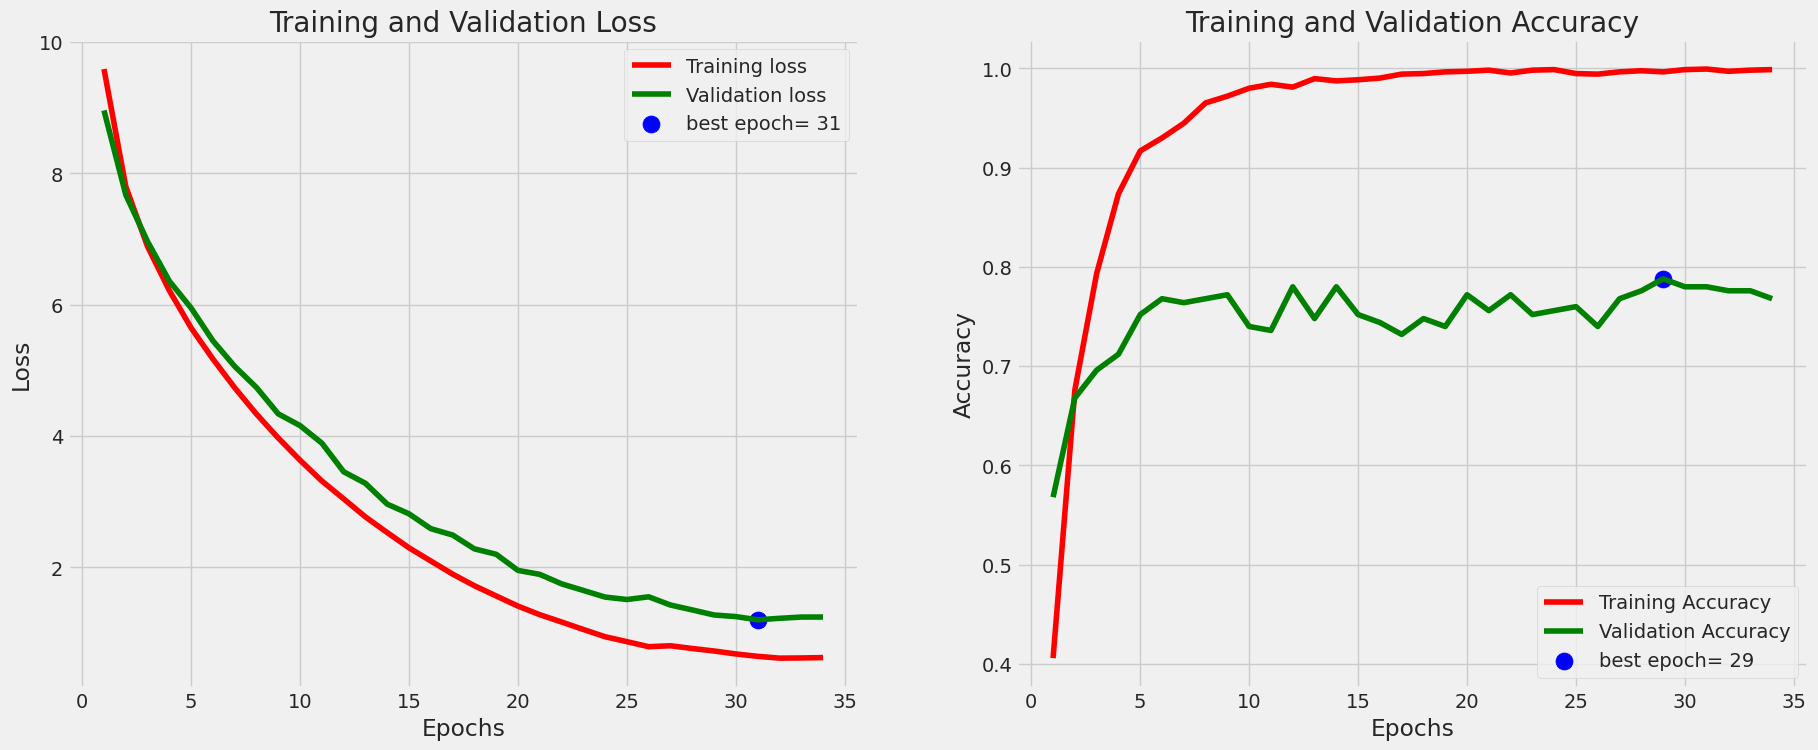
\includegraphics[width=1\textwidth]{./Graphics/training&validation_p1.png}
        \caption{Curva de aprendizaje a lo largo del proceso de entrenamiento del experimento 1.\label{fig:training_validation_loss}}
    \end{center}
\end{figure}

Similar al primer gráfico, en el segundo la pérdida de entrenamiento y validación disminuye, lo que es positivo. La mejor epoch basada en la pérdida de validación es la 19, que ocurre antes que en el primer gráfico, lo que indica una convergencia más rápida. La precisión de entrenamiento también es alta, pero no tan cercana al 100\% como en el primer gráfico, lo que sugiere un menor riesgo de sobre-ajuste. La precisión de validación muestra menos variabilidad y una alineación más cercana con la precisión de entrenamiento, lo que es un indicador de mejor generalización. La diferencia entre la precisión de entrenamiento y validación es menor en comparación con el primer gráfico, lo que sugiere que el modelo podría estar generalizando mejor.

\begin{figure}[ht]%
    \begin{center}
        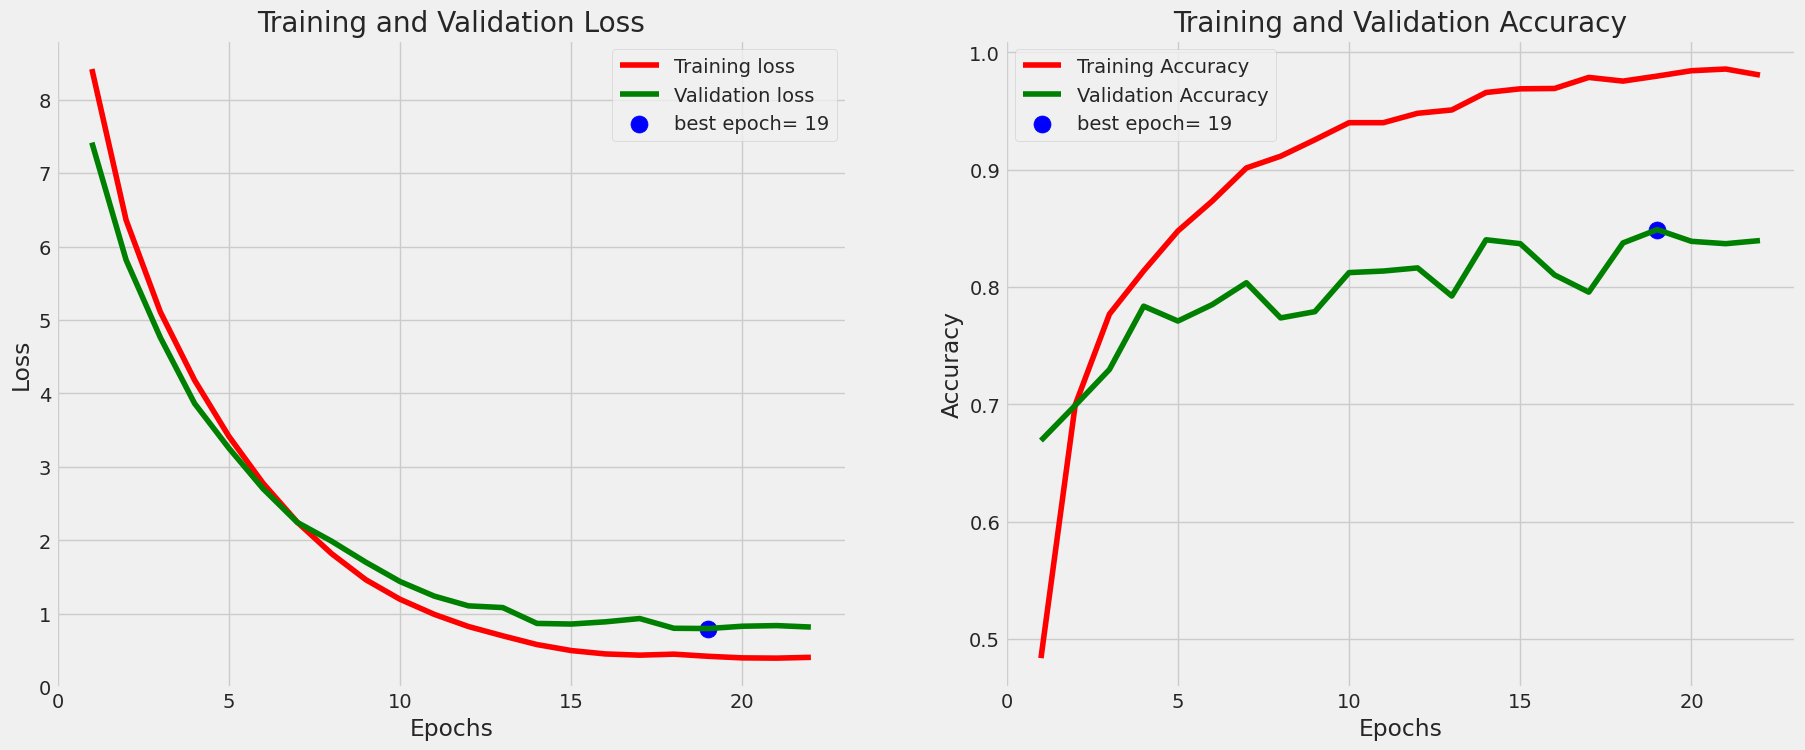
\includegraphics[width=1\textwidth]{./Graphics/training&validation_p3.png}
        \caption{Curva de aprendizaje a lo largo del proceso de entrenamiento del experimento 2.\label{fig:training_validation_loss_p2}}
    \end{center}
\end{figure}

Las figuras 4.1 y 4.2 corresponde a la curva de aprendizaje del experimento 1 y 2 respectivamente.

%-----------------------------------------------------------------------------------
\subsection*{Estadísticas de eficacia}\label{sub:accuracy_statistic_p1}
%-----------------------------------------------------------------------------------
La matriz de confusión proporciona información valiosa sobre el rendimiento del modelo en relación de Actual/Predicho, en términos de su capacidad para clasificar correctamente cada una de las siete clases de cáncer de piel. La diagonal principal de la matriz representa los verdaderos positivos (TP), el número de casos en los que el modelo ha predicho correctamente la clase correspondiente. Los valores fuera de la diagonal principal indican errores de clasificación.

\begin{figure}[ht]
    \centering
    \begin{minipage}{0.45\textwidth}
        \centering
        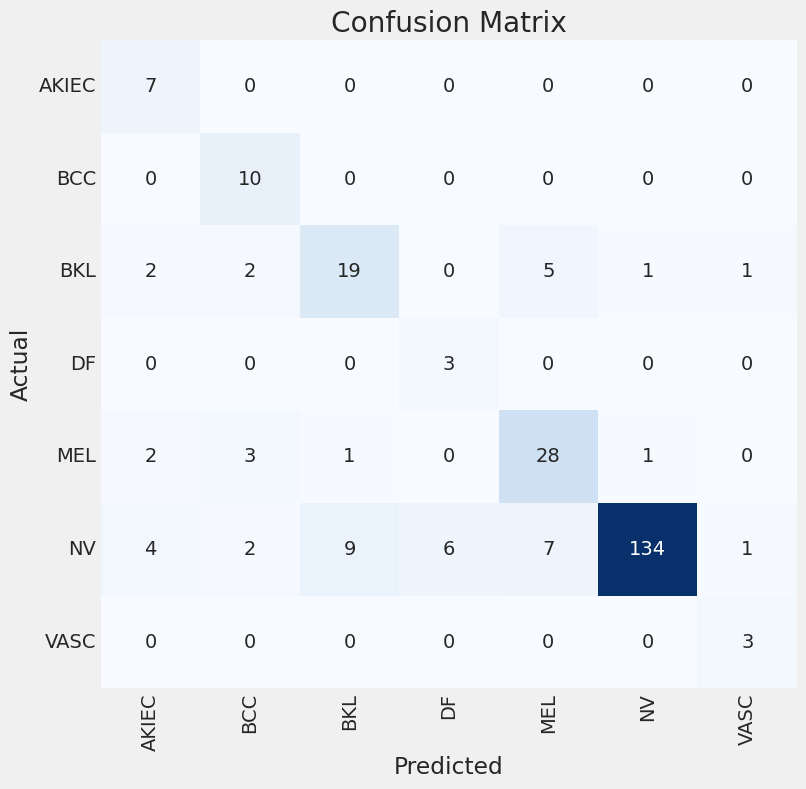
\includegraphics[width=\textwidth]{./Graphics/confussionmatrix_p1.png}
        \caption{Estadísticas de eficacia del modelo al estimar los resultados en el conjunto de pruebas.}
        \label{fig:confussion_matrix_p1}
    \end{minipage}\hfill
    \begin{minipage}{0.45\textwidth}
        \centering
        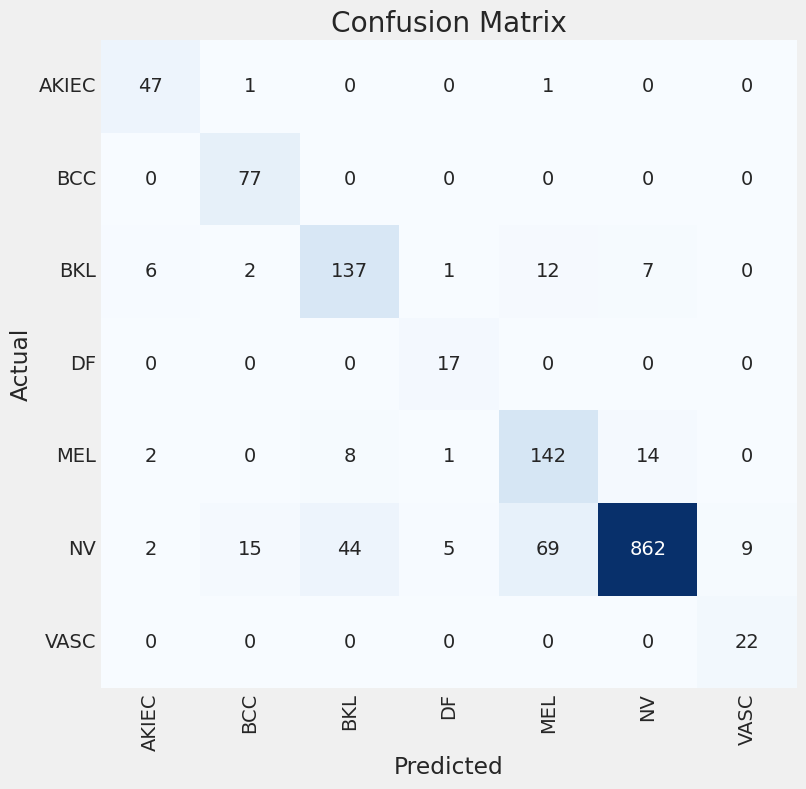
\includegraphics[width=\textwidth]{./Graphics/confussionMatrix_p3.png}
        \caption{Estadísticas de eficacia del modelo al estimar los resultados en el conjunto de pruebas.}
        \label{fig:confussion_matrix_p3}
    \end{minipage}
\end{figure}

En ambas matrices la clase con el mayor número de verdaderos positivos es "NV", en la primera con 134 casos predichos correctamente y en la segunda con 862 casos.

En el caso de 'AKIEC', la tasa de TP mejoró significativamente, pasando de 7 de 300 a 47 de 500. Incluso teniendo en cuenta el aumento del tamaño del conjunto de datos, se trata de una clara mejora. Se observan mejoras similares en otras clases, como 'BCC', 'BKL', 'DF', 'MEL' y 'NV'. La tasa de TP (true positive o verdaderos positivos) ha aumentado no sólo en términos absolutos, sino también proporcionalmente si se tiene en cuenta el mayor tamaño del conjunto de datos. 'VASC' es un caso especial; mientras que la primera matriz no muestra ningún TP y tiene 3 FN (false negative o falsos negativos), la segunda matriz, a pesar de tener un gran número de FP(false positive o falsos positivos) (22), muestra que el modelo ha empezado a reconocer esta clase, cosa que antes no hacía.

En las siguientes figuras se evidencia el margen de error de las clases con mas errores que se obtuvieron en el experimento 1 y 2 respectivamente.

\begin{figure}[ht]%
    \begin{center}
        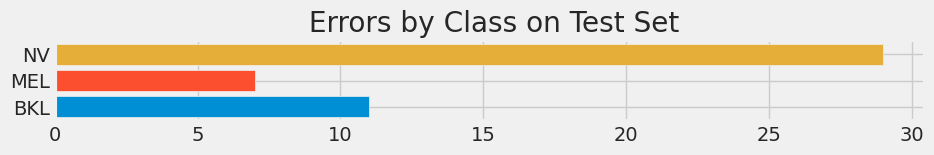
\includegraphics[width=0.8\textwidth]{./Graphics/errorByClass_p1.png}
        \caption{Gráfico de errores por clase en el conjunto de pruebas\label{fig:class_errors_p1}}
    \end{center}
\end{figure} 

\begin{figure}[ht]%
    \begin{center}
        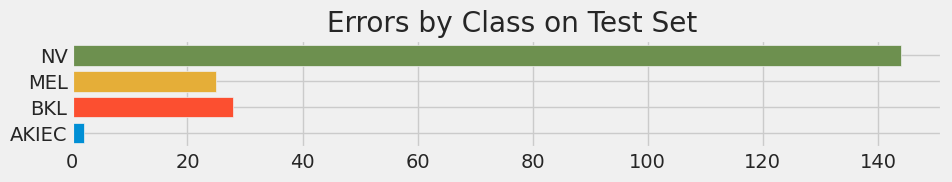
\includegraphics[width=0.8\textwidth]{./Graphics/errorByClass_p3.png}
            \caption{Gráfico de errores por clase en el conjunto de pruebas.\label{fig:class_errors_p3}}
    \end{center}
\end{figure}

En el caso de 'NV', el número de errores del primer gráfico de barras se correlaciona con un conjunto de pruebas en el que el modelo tiene casi las mismas posibilidades de hacer una predicción correcta que de dar un falso positivo. En el segundo gráfico, a pesar del aumento de errores, el modelo tiene la misma proporción de verdaderos positivos que de falsos positivos, lo que sugiere que el rendimiento del modelo se ha mantenido constante en relación con el tamaño del conjunto de datos. 'MEL' y'BKL' muestran un aumento de los errores en el segundo gráfico de barras, pero también es proporcional al aumento del tamaño del conjunto de datos. La proporción de verdaderos positivos frente a falsos positivos sigue siendo la misma.
'AKIEC' presenta un número relativamente pequeño de errores en el segundo gráfico de barras, lo que puede deberse al rendimiento relativamente bueno del modelo en esta clase en el conjunto de datos más grande.

\subsection*{Informe de clasificación}

La tabla siguiente proporcionan una visión cuantitativa de la precisión, el recall (sensibilidad), el puntaje F1 y F2 y el soporte (número de muestras verdaderas) (NM) para cada categoría diagnóstica evaluada. Estos indicadores de rendimiento son esenciales para comprender la capacidad del modelo para identificar correctamente cada condición, así como su confiabilidad general en un conjunto de datos diverso. La métrica de 'Accuracy' refleja la proporción general de predicciones correctas, mientras que los promedios 'Macro' y 'Weighted' proporcionan una perspectiva agregada del rendimiento del modelo, teniendo en cuenta el desequilibrio en el soporte de las clases. 

\begin{table}[ht]
    \small
    \centering
    \caption{Informe de clasificación combinado para los Experimentos 1 y 2.}
    \label{tab:classification_report_combined}
    \begin{tabular}{lcccccccccc}
    \hline
    & \multicolumn{5}{c}{\textbf{Experimento 1}} & \multicolumn{5}{c}{\textbf{Experimento 2}} \\
    \cline{2-10}
    \textbf{Categoría} & \textbf{Acc} & \textbf{Recall} & \textbf{F1} & \textbf{F2} & \textbf{NM} & \textbf{Acc} & \textbf{Recall} & \textbf{F1} & \textbf{F2} & \textbf{NM} \\
    \hline
    AKIEC & 0.47 & 1.00 & 0.64 & 0.816 & 7   & 0.82 & 0.96 & 0.89 & 0.928  & 49 \\
    BCC   & 0.59 & 1.00 & 0.74 & 0.878 & 10  & 0.81 & 1.00 & 0.90 &  0.955 & 77 \\
    BKL   & 0.66 & 0.63 & 0.64 & 0.636 & 30  & 0.72 & 0.83 & 0.77 & 0.805  & 165 \\
    DF    & 0.33 & 1.00 & 0.50 & 0.711 & 3   & 0.71 & 1.00 & 0.83 & 0.924  & 17 \\
    MEL   & 0.70 & 0.80 & 0.75 & 0.778 & 35  & 0.63 & 0.85 & 0.73 & 0.795  & 167 \\
    NV    & 0.99 & 0.82 & 0.90 & 0.849 & 163 & 0.98 & 0.86 & 0.91 & 0.882  & 1006 \\
    VASC  & 0.60 & 1.00 & 0.75 & 0.882 & 3   & 0.71 & 1.00 & 0.83 & 0.924  & 22 \\
    \hline
    \textbf{Acc} & & & 0.81 & & 251 & & & 0.87 & & 1503 \\
    \textbf{M Avg} & 0.62 & 0.89 & 0.70 & & 251 & 0.77 & 0.93 & 0.84 & & 1503 \\
    \textbf{W Avg} & 0.86 & 0.81 & 0.83 & & 251 & 0.89 & 0.87 & 0.87 & & 1503 \\
    \hline
    \end{tabular}
\end{table}

Se añadieron a la tabla 4.3 los campos \textit{Accuracy}, \textit{MacroAvg}(M Avg) y \textit{WeightedAvg}(W Avg) para un mejor análisis de los resultados.

El campo \textit{accuracy} muestra que la precisión mejora de $0.81$ a $0.87$, reflejando un aumento en la capacidad general del modelo para hacer predicciones correctas. El Macro Avg (Promedio Macro) aumento de $0.62$ a $0.77$ en precisión y de $0.70$ a $0.84$ en la puntuación F1, indicando una mejora en el rendimiento medio del modelo a través de todas las categorías. El Weighted Avg (Promedio Ponderado) muestra un incremento de $0.86$ a $0.89$ en precisión y de $0.83$ a $0.87$ en la puntuación F1, mostrando que, teniendo en cuenta el número de muestras (soporte), el rendimiento general del modelo ha mejorado.

Se calcula además $F_{\beta}$ o F2. El cálculo del puntaje F2 es una forma de considerar la precisión y la recuperación (\textit{recall}) en un único número, ponderando uno de estos aspectos más que el otro. En nuestro caso específico le asignamos al recobrado prioridad con respecto a la precisión, dado que en la práctica sería mas importante evitar los falsos positivos. Asignamos $\beta = 2$.

En todas las categorías, el puntaje F2 es mayor en el Experimento 2 que en el Experimento 1. Esto indica que este fue más exitoso en equilibrar la precisión y el recall, especialmente con un enfoque en minimizar los falsos negativos. La mejora general en el Experimento 2 confirma un mejor equilibrio en el conjunto de datos y la efectividad de esto para nuestro propósito.

\section{Observaciones generales entre los experimentos}

En general los experimentos demuestran resultados interesantes en la clasificación. El Experimento 2 muestra mejoras generalizadas en precisión, recall y puntuaciones F1 para la mayoría de las categorías. El soporte aumenta significativamente, lo que indica que se evaluó al modelo con más muestras, proporcionando una base más robusta para la evaluación del rendimiento. A pesar de que el soporte es mayor, lo que generalmente hace más desafiante mantener altas métricas, el Experimento 2 demuestra mejoras en las métricas en general. Este, a diferencia del 1, maneja mejor el desequilibrio de clases, lo que se refleja en una mejor diferenciación entre ciertas categorías diagnósticas, lo que es indicativo de un modelo más preciso y confiable.

\section{Consideraciones finales}
%-----------------------------------------------------------------------------------

Los resultados obtenidos son prometedores y sugieren que los modelos de aprendizaje profundo tienen un potencial considerable para mejorar la precisión y la eficiencia del diagnóstico del cáncer de piel. Tomando como referencia los resultados del experimento 2, se obtuvo una eficacia de clasificación de 87\%, lo cual es bajo con respecto a métodos más robustos mencionados en el estado del arte pero prometedor teniendo en cuenta que los algoritmos desarrollados utilizando EfficientNet obtienen resultados entre 84\% y 86.5\% de eficacia \brackcite{ali2022multiclass}.

Es notable además la importancia para el dataset específico utilizado (HAM10000) de un balance proporcional en el conjunto de datos, dado que se evidencia en los resultados que la desproporción entre los mismos lleva a errores de sobre-ajuste y a un peor rendimiento del modelo.

    \begin{table}[ht]
        \small
        \centering
        \begin{tabular}{|c|c|c|c|c|c|c|c|c|}
        \hline
        \textbf{Epoch} & \textbf{Loss} & \textbf{Acc} & \textbf{V Loss} & \textbf{V Acc} & \textbf{LR} & \textbf{Next LR} & \textbf{Monitor} & \textbf{Duration} \\ \hline
        1 /40  & 9.587  & 40.581 & 8.95658 & 56.800 & 0.00100 & 0.00100 & precisión & 85.25  \\ \hline
        2 /40  & 7.798  & 67.615 & 7.67235 & 66.800 & 0.00100 & 0.00100 & precisión & 21.72  \\ \hline
        3 /40  & 6.884  & 79.340 & 6.96014 & 69.600 & 0.00100 & 0.00100 & precisión & 22.56  \\ \hline
        4 /40  & 6.214  & 87.365 & 6.35865 & 71.200 & 0.00100 & 0.00100 & precisión & 25.81  \\ \hline
        5 /40  & 5.646  & 91.690 & 5.94812 & 75.200 & 0.00100 & 0.00100 & pérdida val. & 23.08  \\ \hline
        6 /40  & 5.172  & 92.999 & 5.44954 & 76.800 & 0.00100 & 0.00100 & pérdida val. & 23.23  \\ \hline
        7 /40  & 4.735  & 94.479 & 5.06016 & 76.400 & 0.00100 & 0.00100 & pérdida val. & 23.19  \\ \hline
        8 /40  & 4.334  & 96.528 & 4.73837 & 76.800 & 0.00100 & 0.00100 & pérdida val. & 22.90  \\ \hline
        9 /40  & 3.969  & 97.211 & 4.33689 & 77.200 & 0.00100 & 0.00100 & pérdida val. & 22.74  \\ \hline
        10 /40 & 3.631  & 98.008 & 4.15826 & 74.000 & 0.00100 & 0.00100 & pérdida val. & 22.56  \\ \hline
        11 /40 & 3.315  & 98.406 & 3.89153 & 73.600 & 0.00100 & 0.00100 & pérdida val. & 23.11  \\ \hline
        12 /40 & 3.044  & 98.122 & 3.45597 & 78.000 & 0.00100 & 0.00100 & pérdida val. & 22.90  \\ \hline
        13 /40 & 2.768  & 98.976 & 3.27968 & 74.800 & 0.00100 & 0.00100 & pérdida val. & 23.01  \\ \hline
        14 /40 & 2.530  & 98.748 & 2.96314 & 78.000 & 0.00100 & 0.00100 & pérdida val. & 22.32  \\ \hline
        15 /40 & 2.298  & 98.862 & 2.81532 & 75.200 & 0.00100 & 0.00100 & pérdida val. & 22.32  \\ \hline
        16 /40 & 2.097  & 99.032 & 2.58953 & 74.400 & 0.00100 & 0.00100 & pérdida val. & 25.73  \\ \hline
        17 /40 & 1.898  & 99.431 & 2.49290 & 73.200 & 0.00100 & 0.00100 & pérdida val. & 23.25  \\ \hline
        18 /40 & 1.721  & 99.488 & 2.28217 & 74.800 & 0.00100 & 0.00100 & pérdida val. & 22.98  \\ \hline
        19 /40 & 1.565  & 99.659 & 2.19958 & 74.000 & 0.00100 & 0.00100 & pérdida val. & 22.36  \\ \hline
        20 /40 & 1.411  & 99.715 & 1.95434 & 77.200 & 0.00100 & 0.00100 & pérdida val. & 22.71  \\ \hline
        21 /40 & 1.280  & 99.829 & 1.89412 & 75.600 & 0.00100 & 0.00100 & pérdida val. & 25.82  \\ \hline
        22 /40 & 1.169  & 99.545 & 1.74949 & 77.200 & 0.00100 & 0.00100 & pérdida val. & 23.20  \\ \hline
        23 /40 & 1.055  & 99.829 & 1.64937 & 75.200 & 0.00100 & 0.00100 & pérdida val. & 23.06  \\ \hline
        24 /40 & 0.944  & 99.886 & 1.54814 & 75.600 & 0.00100 & 0.00100 & pérdida val. & 22.80  \\ \hline
        25 /40 & 0.870  & 99.488 & 1.51110 & 76.000 & 0.00100 & 0.00100 & pérdida val. & 22.87  \\ \hline
        26 /40 & 0.793  & 99.431 & 1.55223 & 74.000 & 0.00100 & 0.00050 & pérdida val. & 22.38  \\ \hline
        27 /40 & 0.807  & 99.659 & 1.42688 & 76.800 & 0.00050 & 0.00050 & pérdida val. & 25.70  \\ \hline
        28 /40 & 0.765  & 99.772 & 1.35257 & 77.600 & 0.00050 & 0.00050 & pérdida val. & 23.38  \\ \hline
        29 /40 & 0.727  & 99.659 & 1.27547 & 78.800 & 0.00050 & 0.00050 & pérdida val. & 22.97  \\ \hline
        30 /40 & 0.682  & 99.886 & 1.25111 & 78.000 & 0.00050 & 0.00050 & pérdida val. & 22.80  \\ \hline
        31 /40 & 0.646  & 99.943 & 1.20186 & 78.000 & 0.00050 & 0.00050 & pérdida val. & 23.36  \\ \hline
        32 /40 & 0.619  & 99.715 & 1.22486 & 77.600 & 0.00050 & 0.00025 & pérdida val. & 23.07  \\ \hline
        33 /40 & 0.621  & 99.829 & 1.24364 & 77.600 & 0.00025 & 0.00013 & pérdida val. & 23.57  \\ \hline
        34 /40 & 0.627  & 99.886 & 1.24470 & 76.800 & 0.00013 & 0.00006 & pérdida val. & 23.30  \\ \hline
        \end{tabular}
        \caption{Resultados del entrenamiento del experimento 1.}
        \label{tab:training_results_b1}
        \end{table}

        
       
            